\documentclass[12pt]{article}
\usepackage{preamble}
\usepackage{longtable}

\geometry{a4paper, left=2.5cm, right=2.5cm, top=2cm, bottom=2.5cm}


\pagestyle{empty}

\chead{
    \begin{minipage}{1\linewidth}
        \begin{wrapfigure}{r}{0pt}
            
\includegraphics[height=1cm]{logo}
        \end{wrapfigure}
        {
            \centering
            \sffamily\scriptsize
            \textbf{
                Санкт-Петербургский национальный исследовательский университет \\
                информационных технологий, механики и оптики}
            %th3p4g
            \vspace{2mm}

            \quad\quad\quad\quad\quad\quad\ \textbf{УЧЕБНЫЙ ЦЕНТР ОБЩЕЙ ФИЗИКИ ФТФ}
        }
    \end{minipage}
}

\begin{document}
    \vspace*{2\baselineskip}

    \thispagestyle{fancy}

    \noindent
    \textbf{Группа} \underline{M3200\hspace{3.85cm}} \hfill \textbf{К работе допущен} \underline{\hspace{4cm}} \\[0.5cm]
    \textbf{Студенты} \underline{Семёнов Д.В. Варакин Г.В. \hspace{0.35cm}} \hfill \textbf{Работа выполнена} \underline{\hspace{4cm}} \\[0.5cm]
    \textbf{Преподаватель} \underline{Шоев В.И.\hspace{0.85cm}} \hfill \textbf{Отчет принят} \underline{\hspace{4.85cm}} \\


    \begin{center}
        {\huge \textbf{Численное моделирование по физике}}

        \smallvspace

        {\Large \textbf{Задание 2, "Частица в конденсаторе"}}

        \smallvspace

        {\Large \textbf{Вариант 15}}
    \end{center}

   \begin{flushleft}
       {\Large \textbf{Условие}}
   \end{flushleft}

    Электрон влетает в цилиндрический конденсатор с начальной скоростью $V$, посередине между обкладками, параллельно образующим цилиндра. При какой минимальной разности потенциалов, приложенной к обкладкам, электрон не успеет вылететь из конденсатора. Краевыми эффектами пренебречь.
    
    Построить графики зависимости $y(x)$, $V_y(t)$, $a_y(t)$, $y(t)$. Координатные оси направлены как показано на рисунке.
    
    Рассчитать время полета $t$ и конечную скорость электрона $V_{\text{кон}}$.


    
    \begin{flushleft}
        {\large \textbf{Используемые константы}}
    \end{flushleft}

    \noindent 
    1. \text{Масса электрона $m_e = 9.109 \cdot 10^{-31}$ кг}
    \smallvspace
    
    \noindent
    2. \text{Заряд электрона $q_e = -1.602 \cdot 10^{-16}$ Кл}
    \smallvspace
    
    \begin{flushleft}
        {\large \textbf{Исходные данные}}
    \end{flushleft}

    \noindent 
    1. \text{Радиус внутренней обкладки $r = 8$ см $= 0.08$ м}
    \smallvspace
    
    \noindent
    2. \text{Радиус внешней обкладки $R = 17$ см $= 0.17$ м}
    \smallvspace
    
    \noindent
    3. \text{Начальная скорость электрона $V = 1.5 \cdot 10^{6} \frac{\text{м}}{\text{с}}$}
    \smallvspace
    
    \noindent
    4. \text{Длина конденсатора $L = 25$ см $= 0.25$ м}
    \smallvspace

    \clearpage

    \begin{flushleft}
        {\large \textbf{Рисунок модели}}
    \end{flushleft}

    \begin{center}
        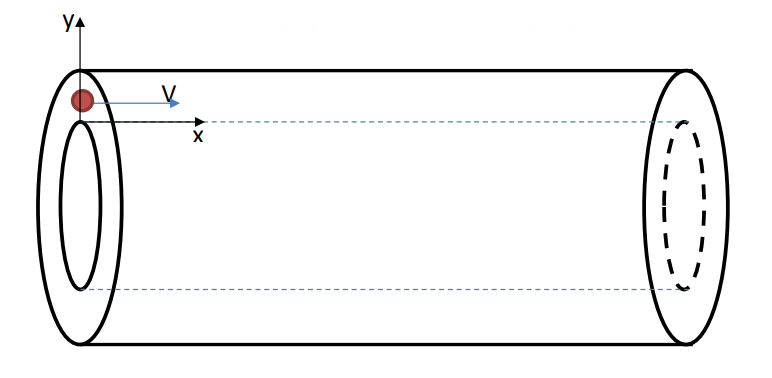
\includegraphics[width=15cm]{images/cond.png}
    \end{center}

    \mediumvspace


    \begin{flushleft}
        {\Large \textbf{Решение}}    
    \end{flushleft}

    Пусть ось $Ox$ совпадает с осью конденсатора.
    
    Разность потенциалов между внутренней и внешней обкладкой положительная. 
    
    Линии напряженности направлены из центра перпендикулярно оси обкладок.

    \smallvspace

    \begin{flushleft}
        {\large \textbf{Вывод формул}}
    \end{flushleft}

    \begin{flushleft}
        {\large Напряжённость в цилиндрическом конденсаторе}
    \end{flushleft}


    Закон Гаусса в интегральной форме:  
    \[
    \oint \vec{E} \cdot d\vec{S} = \frac{Q}{\varepsilon_0}
    \]  

    Где:
   
   - $\oint \vec{E} \cdot d\vec{S}$ — поток электрического поля через поверхность
   
   - $Q$ — заряд, заключённый внутри поверхности
   
   - $\varepsilon_0$ — электрическая постоянная
   
    Рассмотрим цилиндрическую гауссову поверхность радиуса $\rho$ и длины $L$, концентричную внутреннему цилиндру.  
    \[
    \oint \vec{E} \cdot d\vec{S} = E \cdot (2 \pi \rho L),
    \]  
    
    Где:
    
    - $2 \pi \rho L$ — площадь боковой поверхности цилиндра

    \clearpage

    Заряд на внутреннем цилиндре равен $Q = \lambda L$.
    
    Где $\lambda$ — линейная плотность заряда.  
    \[
    E \cdot (2 \pi \rho L) = \frac{\lambda L}{\varepsilon_0}.
    \]
    \[
    E(\rho) = \frac{\lambda}{2 \pi \varepsilon_0 \rho}.
    \]

    \begin{flushleft}
        {\large Разность потенциалов}
    \end{flushleft}

    Разность потенциалов между цилиндрами находится через интеграл:  
    \[
    \Delta \varphi = \varphi_a - \varphi_b = \int_a^b E \, dr.
    \]
 
    \[
    \Delta \varphi = \int_r^R \frac{\lambda}{2 \pi \varepsilon_0 \rho} \, d\rho.
    \]

    \[
    \Delta \varphi = \frac{\lambda}{2 \pi \varepsilon_0} \int_r^R \frac{1}{\rho} \, d\rho = \frac{\lambda}{2 \pi \varepsilon_0} \left[ \ln \rho \right]_r^R.
    \]

    \[
    \Delta \varphi = \frac{\lambda}{2 \pi \varepsilon_0} \ln\frac{R}{r}.
    \]

    \begin{flushleft}
        {\large Связь напряжённости и разности потенциалов}
    \end{flushleft}

    Из последней формулы выразим линейную плотность заряда:

   \[
   \lambda = \frac{\Delta \varphi \cdot 2 \pi \varepsilon_0}{\ln\frac{R}{r}}.
   \]

    Подставим в формулу напряжённости:  
   \[
   E(\rho) = \frac{\Delta \varphi \cdot 2 \pi \varepsilon_0}{2 \pi \varepsilon_0 \rho \ln\frac{R}{r}}.
   \]
  
   \[
   E(\rho) = \frac{\Delta \varphi}{\rho \ln\frac{R}{r}}.
   \] 

   В наших обозначаниях можно перейти к:
   \[
   E(y) = \frac{\Delta \varphi}{y \ln\frac{R}{r}}.
   \]

   \begin{flushleft}
        {\large Ускорение электрона}
    \end{flushleft}

    По Второму Закону Ньютона:

    \[
    a_y(y) = \frac{F}{m_e} = \frac{q_eE(y)}{m_e} = \frac{q_e\Delta \varphi}{m_eyln\frac{R}{r}}
    \]

    \clearpage

    \begin{flushleft}
        {\large \textbf{Моделирование задачи}}
    \end{flushleft}

    Если электрон не успевает вылетить из конденсатора, то он сталкивается с одной из его обкладок. Обозначим за $t$ время полета электрона до столкновения.

    Тогда получаем систему:

    \[
    \begin{cases}
        \frac{d^2 y}{dt^2} = \frac{q_e \Delta \varphi}{m_ey\ln\frac{R}{r}}, \\
        y(0) = \frac{R + r}{2}, \\
        v_y(0) = 0, \\
        y(t) = r, \\
        V \cdot t < L
    \end{cases}
    \]

    Напишем код на языке программирования Python, который будет решать следующую задачу. С некоторым маленьким шагом $dt$ (положим, $10^{-14}$) будем при помощи метода Эйлера (метод прямоугольников) считать интегралы до некоторого $t$. Первое значение $\Delta \varphi$, для когорого существует $t$, такое, что будет верна система выше - искомое. Для подбора $\Delta \varphi$ воспользуемся вещественным двоичным поиском.

    В результате выполнения программы получены следующие результаты: $\Delta \varphi = 1.62575 \text{В}$, $t = 1.66667 \text{с}$, $V_{\text{кон}} = -0.581861 \cdot 10^5$

     Добавим в код построение графиков зависимостей $y(x)$, $v_y(t)$, $a_y(t)$, $y(t)$.

    \smallvspace

    \begin{center}
        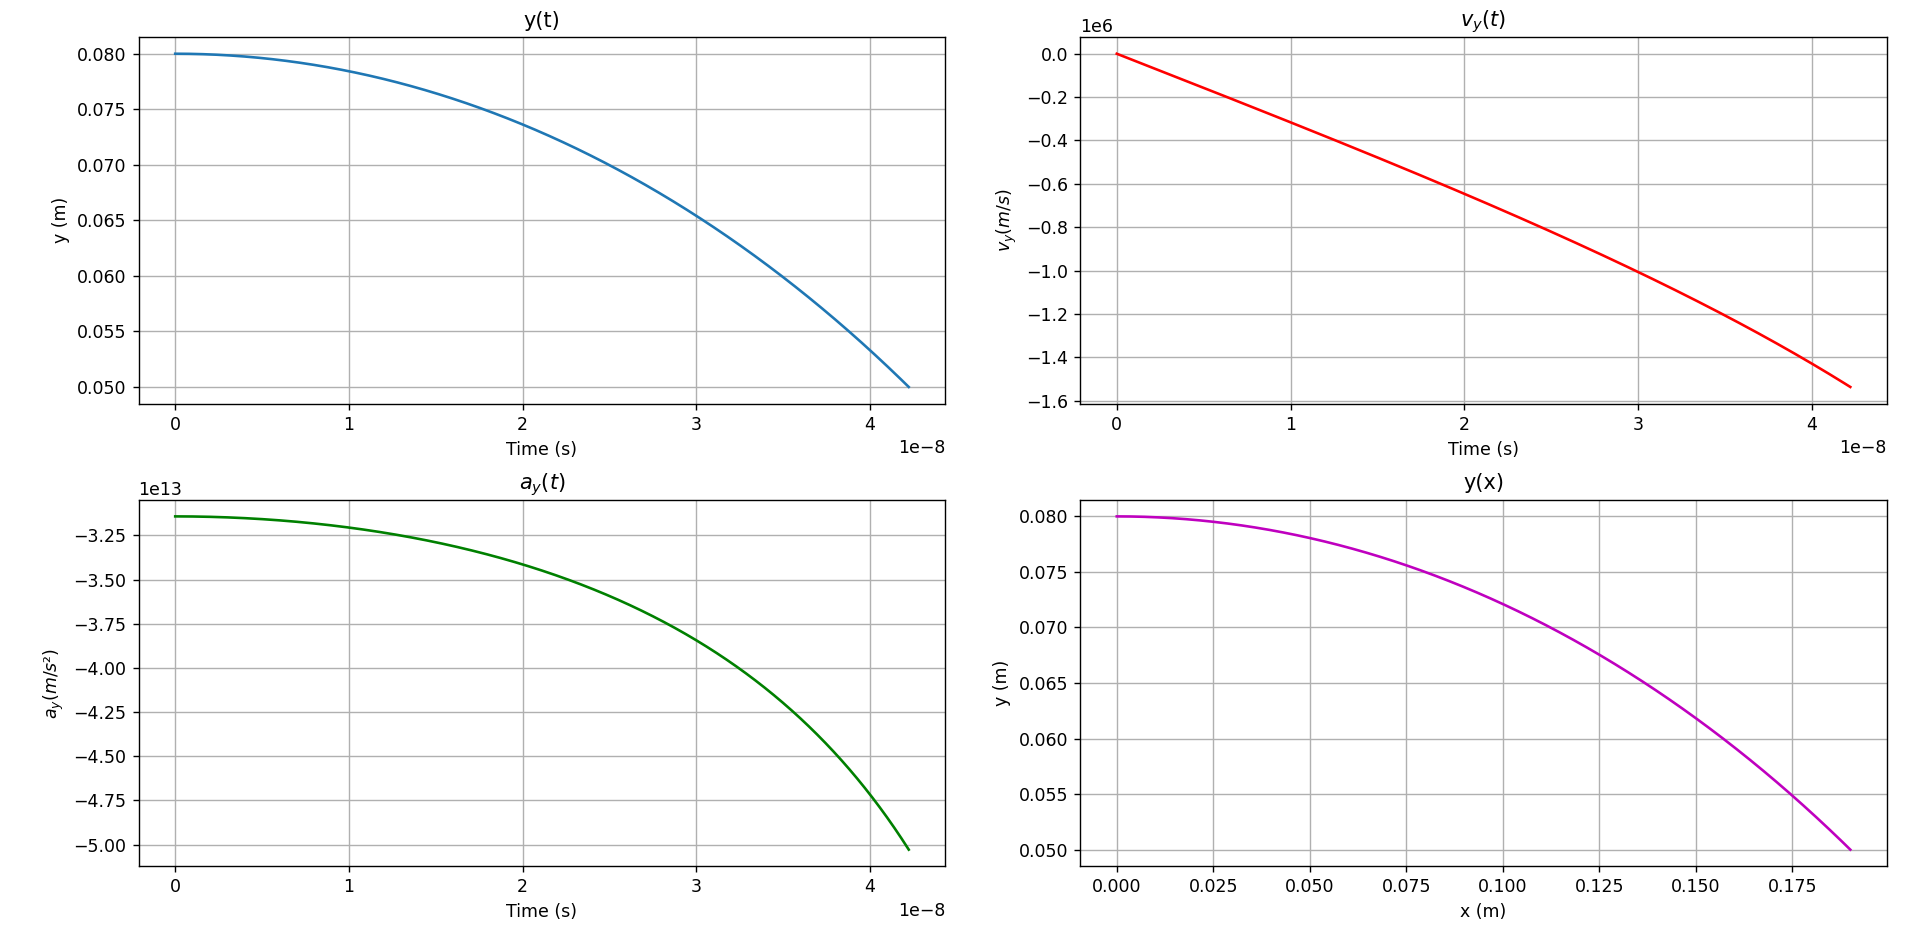
\includegraphics[width=15cm]{images/Graphics.png}

        \smallvspace

        \textit{График 1.} Зависимость $y(x), y(t), v_y(t), a_y(t)$
    \end{center}

    \begin{flushleft}
       {\Large \textbf{Вывод}}
   \end{flushleft}

    В ходе работы было произведено численное моделирование полёта электрона в цилиндрическом конденсаторе. В результате, было получено, что электрон не успеет вылететь из конденсатора при данных условиях, если разность потенциалов, приложенная к обкладкам, будет равна $\Delta \varphi = 1.62575 \text{В}$.
\end{document}